\subsection{Pile-up}
\label{sec:GBJ1:Pileup}



Two effects from pile-up are studied; in-time pile-up and out-of-time (OOT) pile-up.
In-time pile-up is additional proton-proton interactions in the event and is dependent on the number of primary vertices.
Out-of-time pile-up is additional energy coming from previous bunch collisions and depends on both the number of primary vertices of the previous bunches and the bunch spacing. 
Both have the effect of adding additional energy to the event, which can affect the gap fraction.

Requiring one primary vertex will reduce the effect of in-time pile-up. 
The effect of the OOT pile-up and the residual in-time pile-up are assessed by comparing the average gap fraction for different pile-up conditions.
Table \ref{GBJ1:VertexAve} shows that the average number of primary vertices for different periods increases throughout 2010 data taking. 
The main changes in the bunch spacing are in period E, where it was partially reduced, and in period G, where bunch trains with 150~ns bunch spacing were introduced.


The data periods are combined into two different bunch spacing conditions.
In periods B-D the bunch spacing was large, and so the effect of OOT pile-up is expected to be small.
In periods E-I, the bunch spacing was smaller, especially from period G onwards.
It is expected that the effect of OOT pile-up will be larger in this period.
The effect of OOT pile-up is assessed by considering the average gap fraction for different slices in \dy{} and \ptb{} as a function of data period.
The periods B-D and E-I are separately fitted with a constant, and the differences between these fits are used to assess the effect. 

To assess the residual effect from in-time pile-up, the average gap fraction for different slices in \dy{} and \ptb{} as a function of data period is fitted with
\begin{equation}                              
y = A + B x,
\label{GBJ1:Fit1}
\end{equation}
where $x$ is the data period.
If there is no period dependence, the gradient $B$ is constsitant with zero. 


Figures \ref{GBJ1:GFAve6070} - \ref{GBJ1:GFAve150180} show the average gap fraction as a function of period for various \dy{} and \ptb{} slices with fits to the two different OOT pile-up conditions, periods B-D and E-I, with a simple $y = A$ fit. 
Figure \ref{GBJ1:GFAve6070} shows this for a low \ptb{} range of 60--70 GeV for (a) $1<\dy{}<2$, (b) $2<\dy{}<3$ and (c) $3<\dy{}<5$.
The fit for the periods EFGHI is level with the period BCD for the lowest \dy{} range, $0.2$ above for the medium \dy{} range and $0.1$ below for the \dy{} range.
For this \ptb{} range no trend is observed.
Figures \ref{GBJ1:GFAve90120} and \ref{GBJ1:GFAve150180} show a similar lack of trend and difference within $0.2$.
These results would indicate that there is no significant effect from OOT pile-up. 


Table \ref{GBJ1:GFAveTable} shows the result of fiting the function in Equation \ref{GBJ1:Fit1} to the various \dy{} and \ptb{} slices. 
The fits from the period-dependent function show that the gradient of the line, $B$, is consistent, within statistical uncertainties, with zero for almost all slices. 
These two methods have shown that after the primary vertex cut, the effect of pile-up is negligible. 
 
\begin{table}
\begin{center}
\begin{tabular}{|c|c|}
\hline
Period&$\langle N_{PV} \rangle$\\
\hline
B&1.07\\
C&1.06\\
D&1.57\\
E&1.89\\
F&2.18\\
G&2.46\\
H&2.33\\
I&2.78\\
\hline
\end{tabular}
\caption[Average number of primary vertices for different data periods]{ 
Average number of vertices ($\langle N_{PV} \rangle$) for the different data taking periods.
\label{GBJ1:VertexAve}}
\end{center}
\end{table}

\begin{figure}
\centering
        \begin{subfigure}[b]{0.5\textwidth}
                \centering
                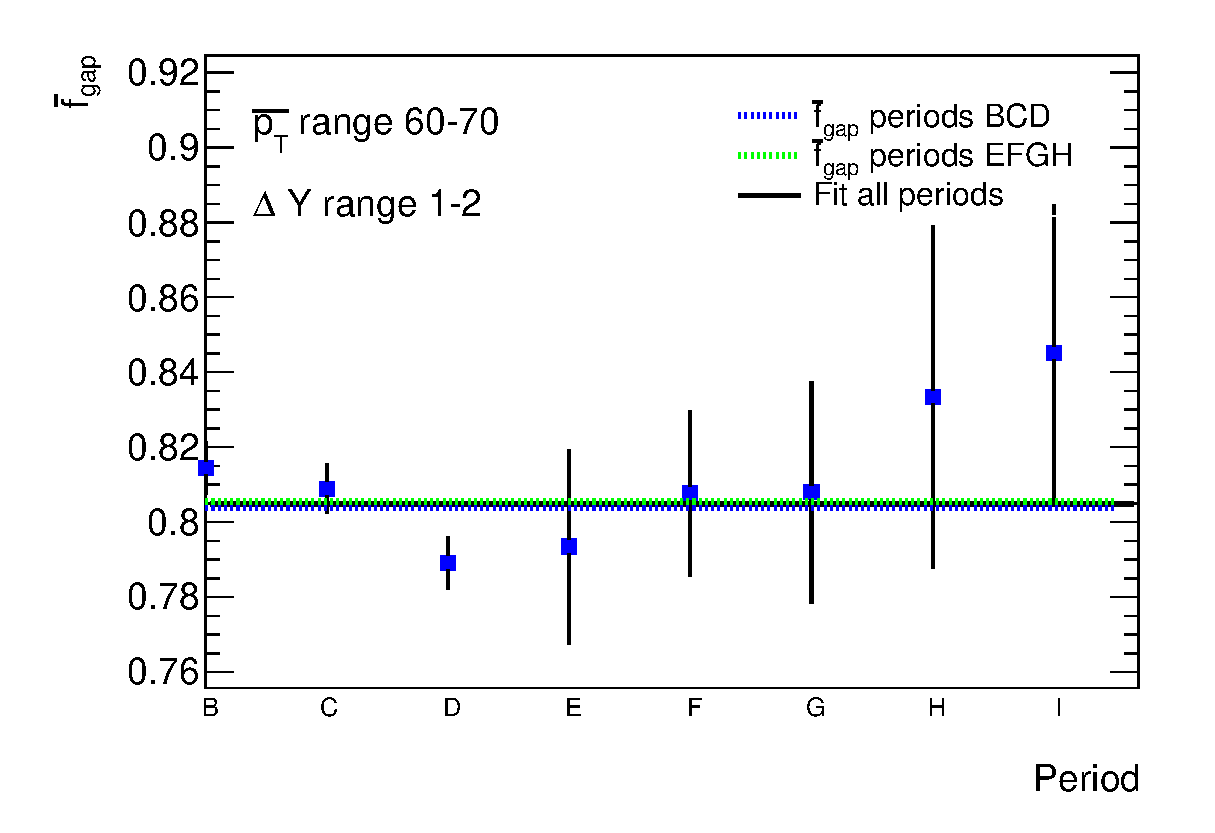
\includegraphics[width=\textwidth]{figures/GBJ1/DataStability/Pileup/GFAve_060_70_1-2_exclusive.eps}
        \end{subfigure}%
        \begin{subfigure}[b]{0.5\textwidth}
                \centering
                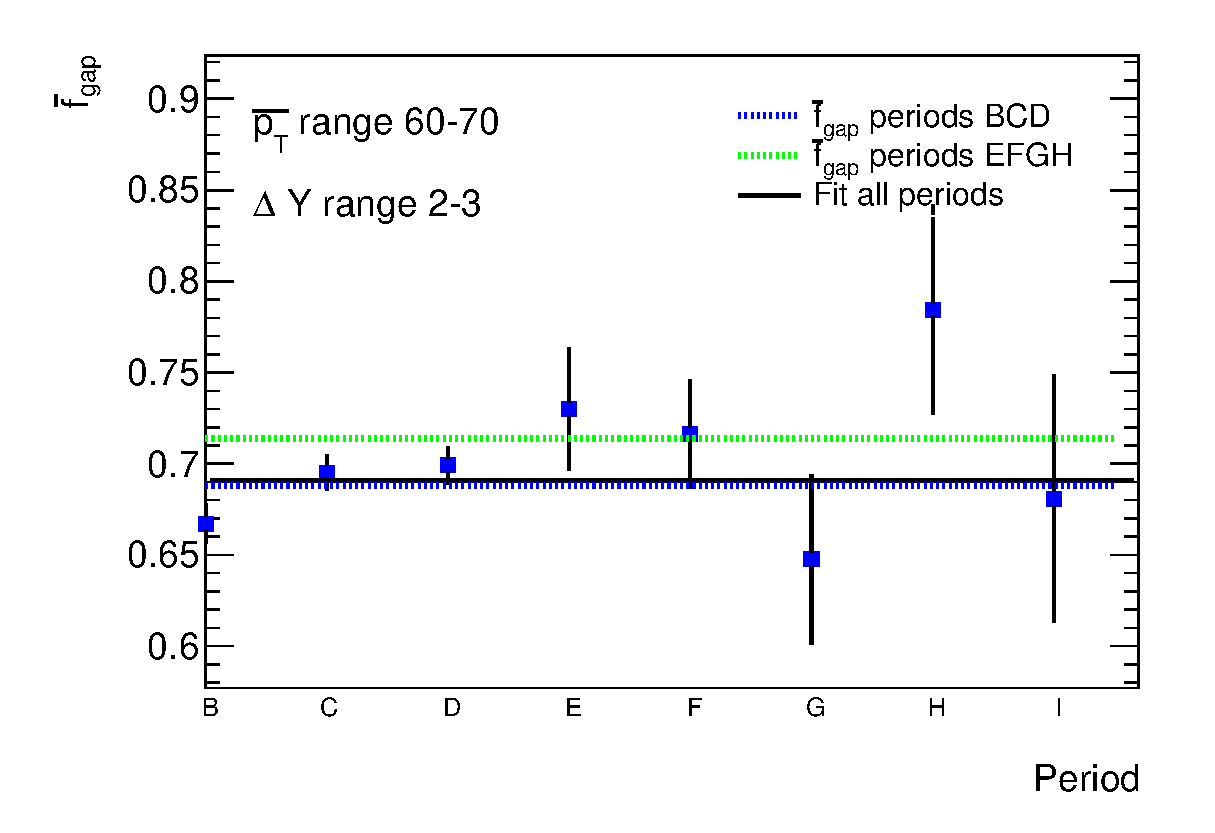
\includegraphics[width=\textwidth]{figures/GBJ1/DataStability/Pileup/GFAve_060_70_2-3_exclusive.eps}
        \end{subfigure}%

        \begin{subfigure}[b]{0.5\textwidth}
                \centering
                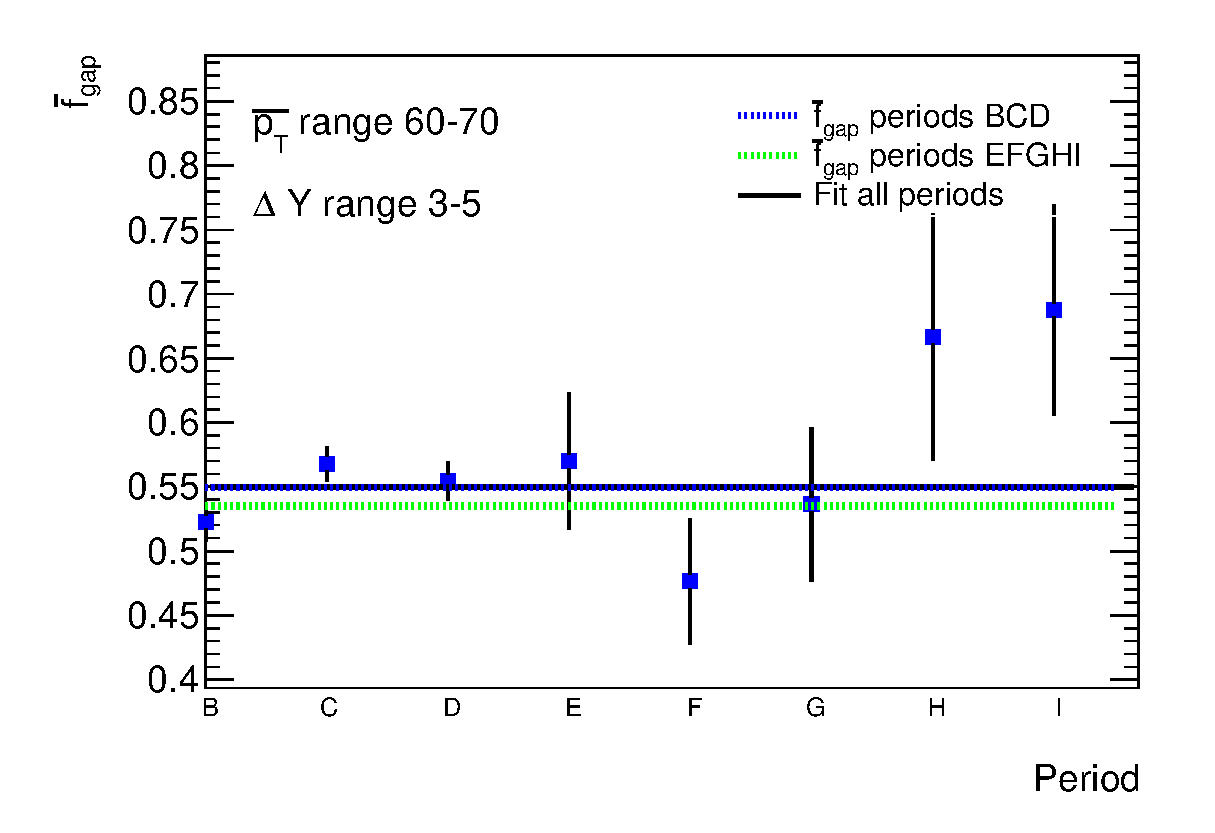
\includegraphics[width=\textwidth]{figures/GBJ1/DataStability/Pileup/GFAve_060_70_3-5_exclusive.eps}
        \end{subfigure}%

\caption[Average gap fraction versus period for $60<\ptb{}<70$ GeV]{
Average gap fraction with $60<\ptb{}<70$ GeV and (a) $1<\dy{}<2$, (b) $2<\dy{}<3$  and (c) $3<\dy{}<5$. 
Each set of average gap fractions have been fitted with three constants; one for periods B-D, one for periods E-I and one for all periods.
\label{GBJ1:GFAve6070}}
\end{figure}



\begin{figure}
\centering
        \begin{subfigure}[b]{0.5\textwidth}
                \centering
                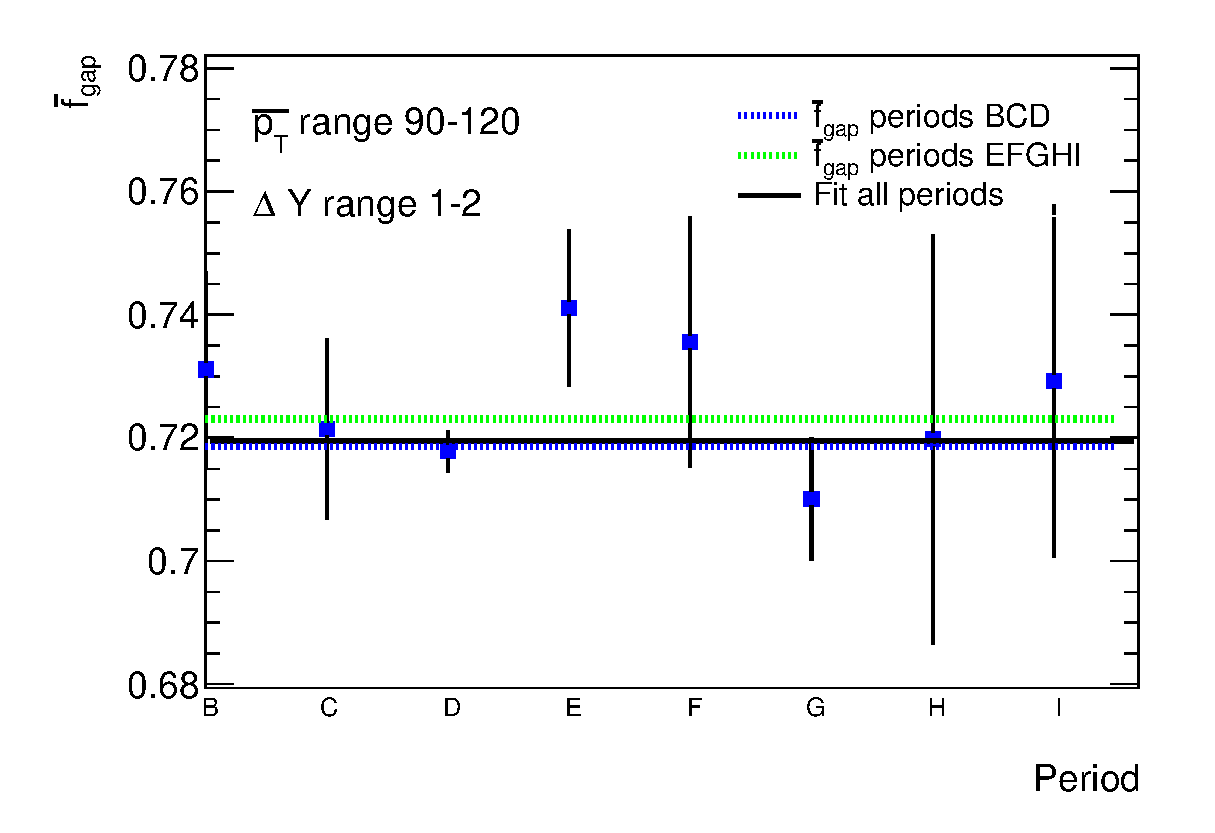
\includegraphics[width=\textwidth]{figures/GBJ1/DataStability/Pileup/GFAve_090_120_1-2_exclusive.eps}
        \end{subfigure}%
        \begin{subfigure}[b]{0.5\textwidth}
                \centering
                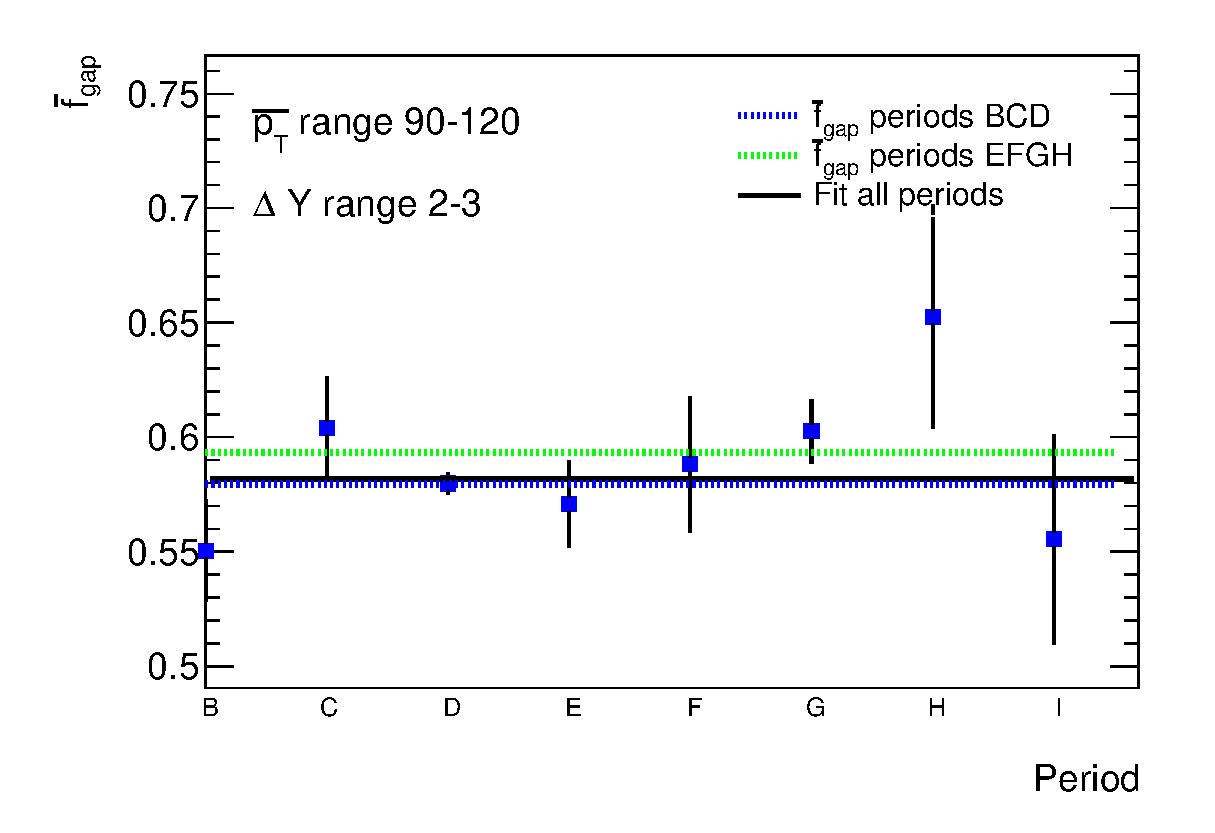
\includegraphics[width=\textwidth]{figures/GBJ1/DataStability/Pileup/GFAve_090_120_2-3_exclusive.eps}
        \end{subfigure}%

        \begin{subfigure}[b]{0.5\textwidth}
                \centering
                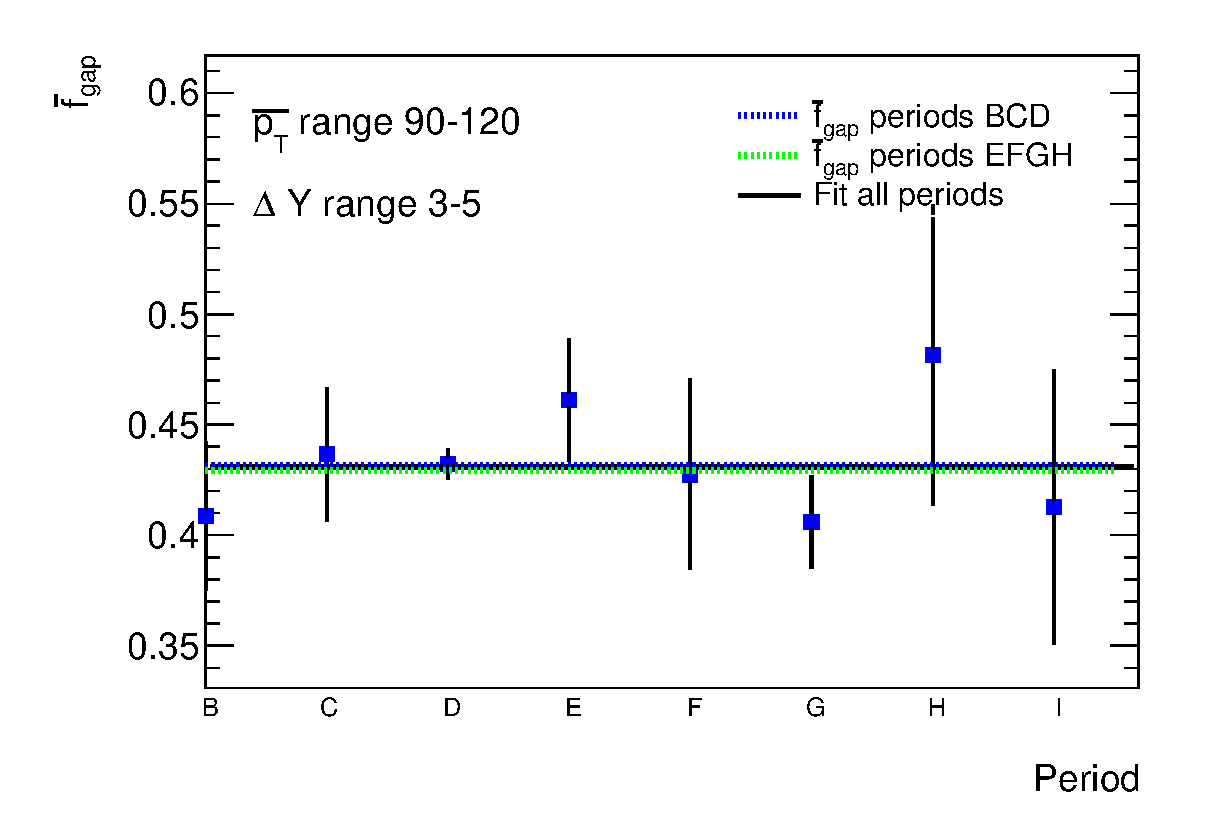
\includegraphics[width=\textwidth]{figures/GBJ1/DataStability/Pileup/GFAve_090_120_3-5_exclusive.eps}
        \end{subfigure}%
\caption[Average gap fraction versus period for $90<\ptb{}<120$ GeV]{
Average gap fraction with $90<\ptb{}<120$ GeV and (a) $1<\dy{}<2$, (b) $2<\dy{}<3$  and (c) $3<\dy{}<5$. 
Each set of average gap fractions have been fitted with three constants; one for periods B-D, one for periods E-I and one for all periods.
\label{GBJ1:GFAve90120}}
\end{figure}



\begin{figure}
\centering
        \begin{subfigure}[b]{0.5\textwidth}
                \centering
                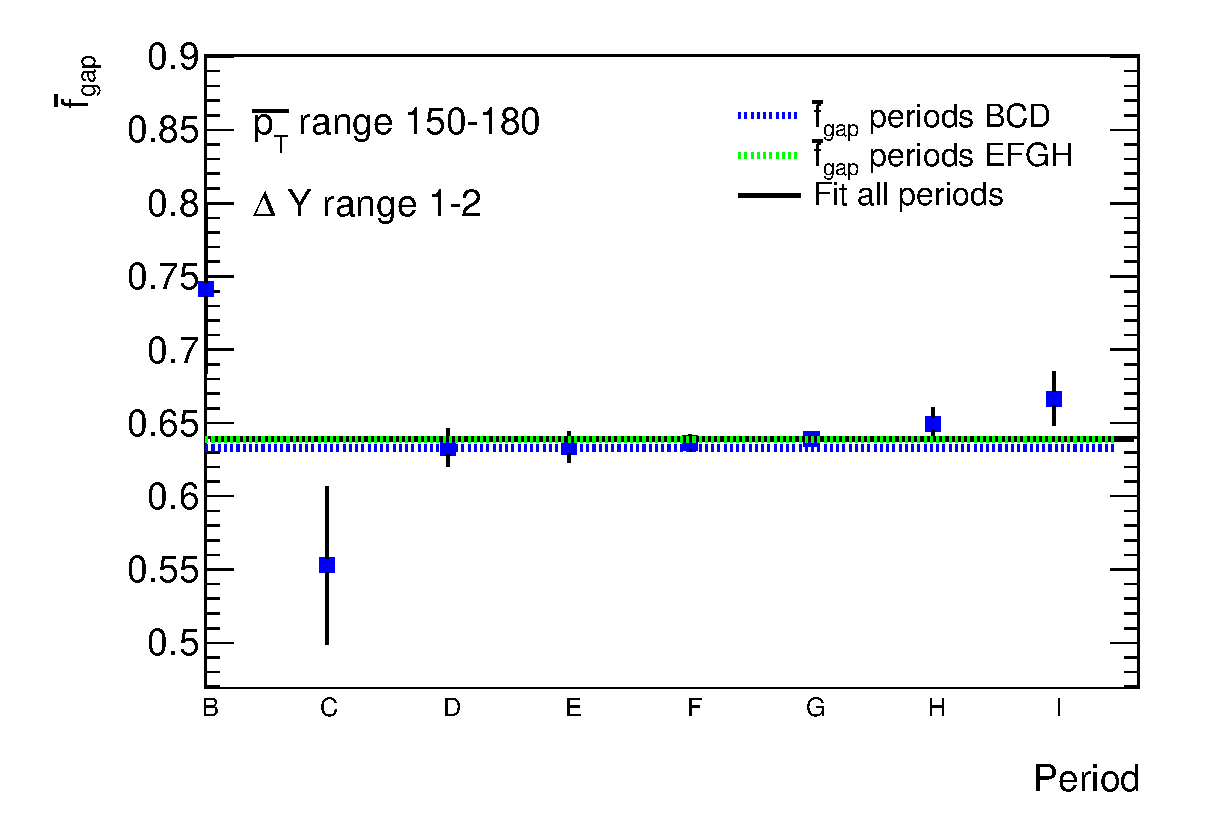
\includegraphics[width=\textwidth]{figures/GBJ1/DataStability/Pileup/GFAve_150_180_1-2_exclusive.eps}
        \end{subfigure}%
        \begin{subfigure}[b]{0.5\textwidth}
                \centering
                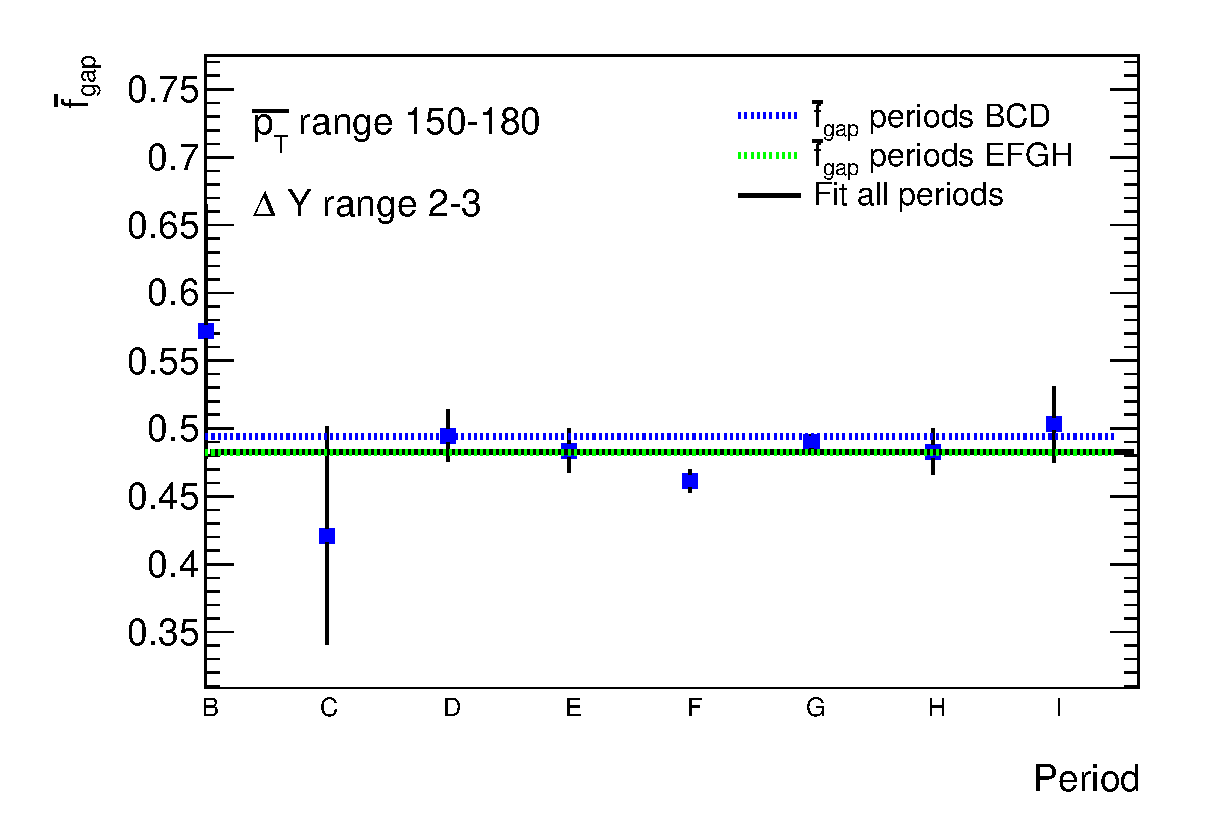
\includegraphics[width=\textwidth]{figures/GBJ1/DataStability/Pileup/GFAve_150_180_2-3_exclusive.eps}
        \end{subfigure}%

        \begin{subfigure}[b]{0.5\textwidth}
                \centering
                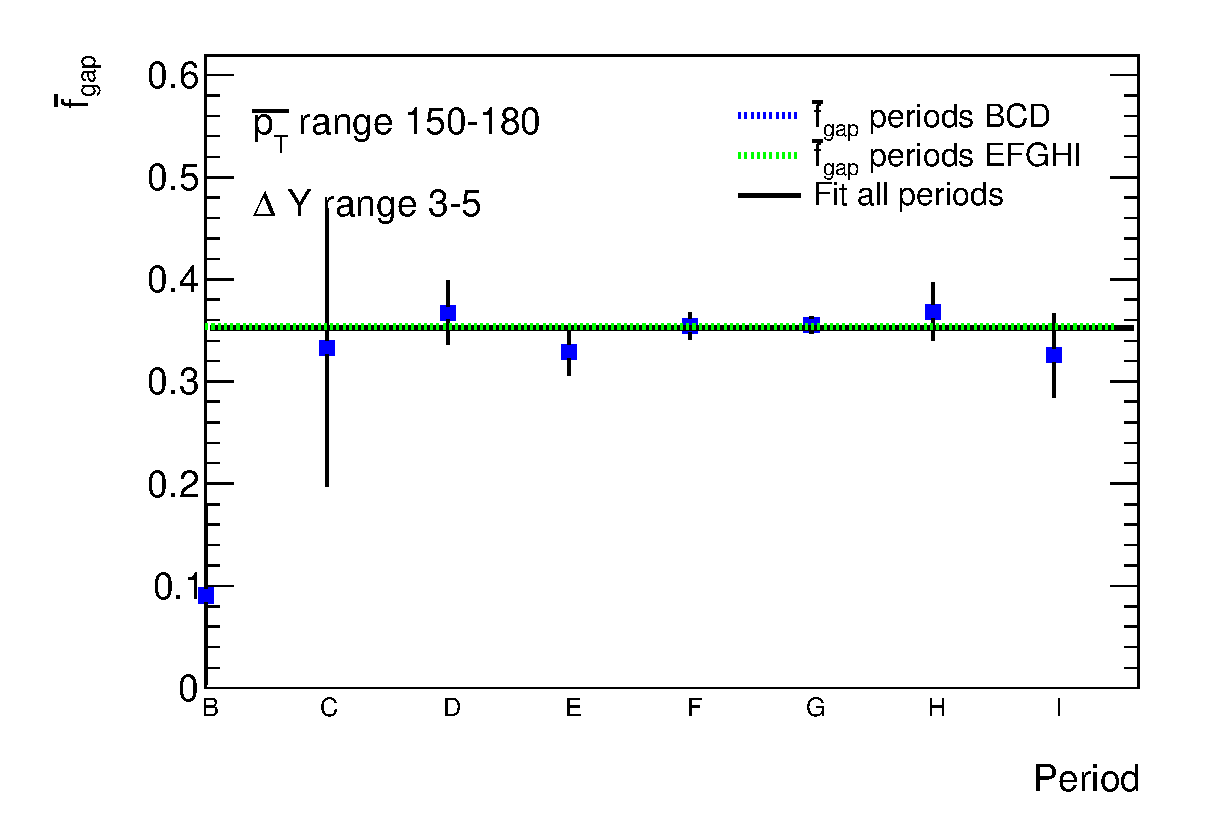
\includegraphics[width=\textwidth]{figures/GBJ1/DataStability/Pileup/GFAve_150_180_3-5_exclusive.eps}
        \end{subfigure}%
\caption[Average gap fraction versus period for $150<\ptb{}<180$ GeV]{
Average gap fraction with $150<\ptb{}<180$ GeV and (a) $1<\dy{}<2$, (b) $2<\dy{}<3$  and (c) $3<\dy{}<5$. 
Each set of average gap fractions have been fitted with three constants; one for periods B-D, one for periods E-I and one for all periods.
\label{GBJ1:GFAve150180}}
\end{figure}



\begin{table}
%\footnotesize 
%\small
\centering
\begin{tabular}{ | c | c | c | c | c | c |  }
\hline
\hline
\dy{} & \ptb{} & $\bar{f}_{gap}$ & \multicolumn{3}{|c|}{$y = A + Bx$}\\
   & GeV& Periods B-D &$A$&$B / 10^{-3}$&$\chi^{2}$/NDF\\
%\dy{} & $\ptb{} [GeV]$ & $\bar{f}_{gap}$ & b & c & d & e & f  \\
\hline
\input{figures/GBJ1/DataStability/Pileup/AveGFTable2.txt}
\hline
\hline
\end{tabular}
\caption[Results from period dependent and period independent fits to the average gap fraction as a function of period]{
The results from fits to the period dependent function in Equation \ref{GBJ1:Fit1} for various slices of \dy{} and \ptb{}.
\label{GBJ1:GFAveTable}}
\end{table}

